\chapter{Technology of ice reservoirs}
\label{chap:tech}

\cleanchapterquote{In building ice stupas, it is necessary to engage enough workforce to extract the water over
	long distances and to keep water flowing in cold temperatures.}{Marcus Nüsser}{(Professor, South Asia Institute)}

Mountains are expected to experience stronger warming than lowlands
\citep{ragettliContrastingClimateChange2016}, which makes them particularly prone to negative effects on
water resources, including the loss of water-regulation capacity.

Especially in the cold-arid Trans-Himalayan region of Ladakh, meltwater supply from the cryosphere is of utmost
importance for irrigated agriculture in spring and summer, when water demand is highest
\citep{nusserCryosphereFedIrrigationNetworks2019}. Due to its short growing period, central Ladakh is a
single-cropping area with barley and wheat as important staples, complemented with vegetables, pulses, and oil
seeds \citep{nusserSociohydrologyArtificialGlaciers2019}. Depending on the altitude, irrigation with complete
flooding of fields (approximately 2–5-cm water column) starts between March and April, prior to the melting of
high-altitude glaciers. This results in increased demand during a period of reduced supply at the onset of the
agricultural season.

These trends stress the importance of increased water storage capacity for glacierized catchments as a pathway
for climate adaptation. Because of the challenges and cost related to conventional storage efforts, AIRs can be
a better tool to adapt against reduced glacial runoff. 

%AIRs, located at much lower altitudes than naturally occuring glaciers, serve to bridge the critical gap in
%water availability by providing meltwater earlier in the agricultural season. Such ice reservoirs utilize the
%hydrological process of icing under local conditions of frequent freeze--thaw cycles to capture water for
%seasonal storage. These water storage structures do not freeze from the top down but are produced
%through sequential freezing of thin layers of water, creating superimposed sheets of ice.



%\begin{figure}[htb]
%	\centering
	%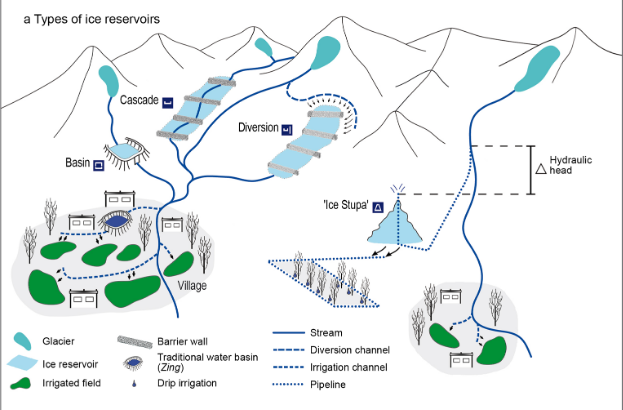
\includegraphics[width=\textwidth]{figs/AIR_designs}
	%\caption{Different types of ice reservoirs. Adapted from \citet{nusserSociohydrologyArtificialGlaciers2019}.}
	%\label{fig:AIRdesigns}
 %\end{figure}

%The different construction strategies of ice reservoirs are described (Fig.
 %\ref{fig:AIRdesigns}) in this chapter; so is the enhancement of AIR models to propose engineering options that 
 %reduce their water losses and maintenance requirements.

\section{Types of ice reservoirs}

\subsection{Ice terraces}

According to oral history and satellite imagery from 1969, the first ice terraces date back over 50 years and can
be found in Phuktse and Igoo villages in Ladakh. Over the past 30 years, 14 ice terraces have been constructed in central Ladakh,
located in tributary valleys of the Indus \citep{norphelArtificialGlacierHigh2009,
	nusserSociohydrologyArtificialGlaciers2019}. Chewang Norphel, a well-known engineer of the Leh Nutrition
Project, introduced this practice to Ladakh \citep{vinceGlacierMan2009}.

\begin{figure}[htb]
	\centering
	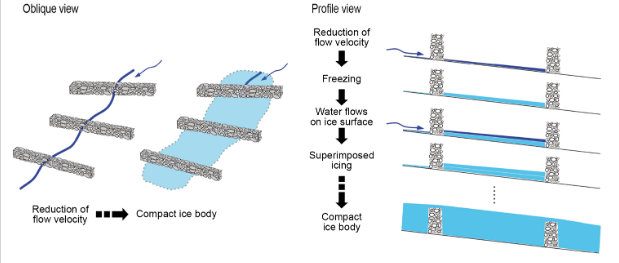
\includegraphics[width=\textwidth]{figs/IT_science.png}

	\caption{ The process of ice accumulation for ice terraces. Adapted from
		\citet{nusserSociohydrologyArtificialGlaciers2019}.}

	\label{fig:ITscience}
\end{figure}

Two distinct types of ice terraces can be differentiated, with site-specific modifications. The first type is built as cascades on perennial streams. A series of loose-rock walls on
the river bed reduces flow velocity but still lets water pass through. Such cascades allow flowing water to
freeze on exposed surfaces and form superimposed ice layers when temperatures drop (Fig.
\ref{fig:ITscience}). An example of this is illustrated in Fig. \ref{fig:ITexample}.

The second type diverts water from streams with higher flow velocity to small side valleys, shaded by
surrounding mountains. This design allows to integrate higher slope positions for additional ice formation and
consists of a series of partially cemented stone walls across the stream bed. Their dimensions are adjusted
based on the valley topography. Water for the ice terrace is obtained through a long diversion channel.


\begin{figure}[htb]
	\centering
	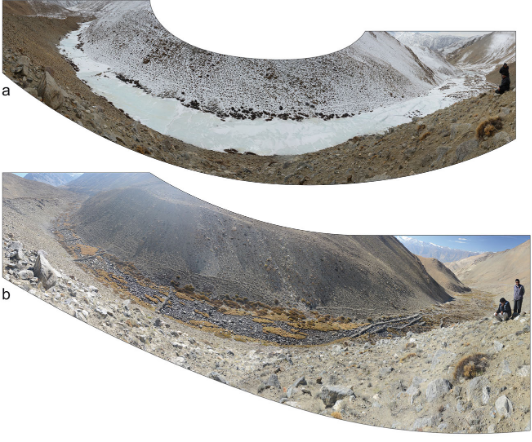
\includegraphics[width=\textwidth]{figs/IT_example.png}
	\caption{Ice terrace of Phuktse, viewpoint 4430 m. (a) February, 2014 and (b) October, 2014. Adapted from:
		\citet{nusserSociohydrologyArtificialGlaciers2019}.}
	\label{fig:ITexample}
\end{figure}

% The following construction guidelines are applied depending on the terrain of the construction site
% \citep{norphelSnowWaterHarvesting2015}:
%
% \begin{itemize}
%
% 	\item If the section of the stream is very wide with a mild slope, then stone walls are
% 	      constructed parallel to each other in a series. Number and dimensions of ice-retaining walls depend on
% 	      the water flow available in the main stream during peak winter.
%
% 	\item If the section of the stream is narrow with a steep gradient, then this needs to be diverted to a shady area
% 	      by constructing a gravitational channel with sufficient slope. Inclination should be gradually reduced upon reaching the ice terrace site, 
% 	      allowing water to flow through small outlets and thus accelerating freezing. Stone
% 	      walls need to be constructed parallel to the channel in series, according to the natural slope of the terrain.
% 	      The steeper the terrain, the smaller the distance and slope between bunds.
%
% \end{itemize}


\subsubsection{Water storage and cost}

The volume variations of ice terraces within Ladakh range from 510 $m^3$ to 81,040 $m^3$, highlighting
the importance of local topography and microclimate in their formation
\citep{nusserSociohydrologyArtificialGlaciers2019, norphelSnowWaterHarvesting2015}. The cost of construction
depends on the size and number of stone walls required. The estimated material costs of ice terraces vary between
4600 and 15,330 USD \citep{nusserSociohydrologyArtificialGlaciers2019}. The building of ice terraces also relies
on the participation of village communities for construction and maintenance.

\subsection{Ice stupas}

\begin{figure}[htb]
	\centering
	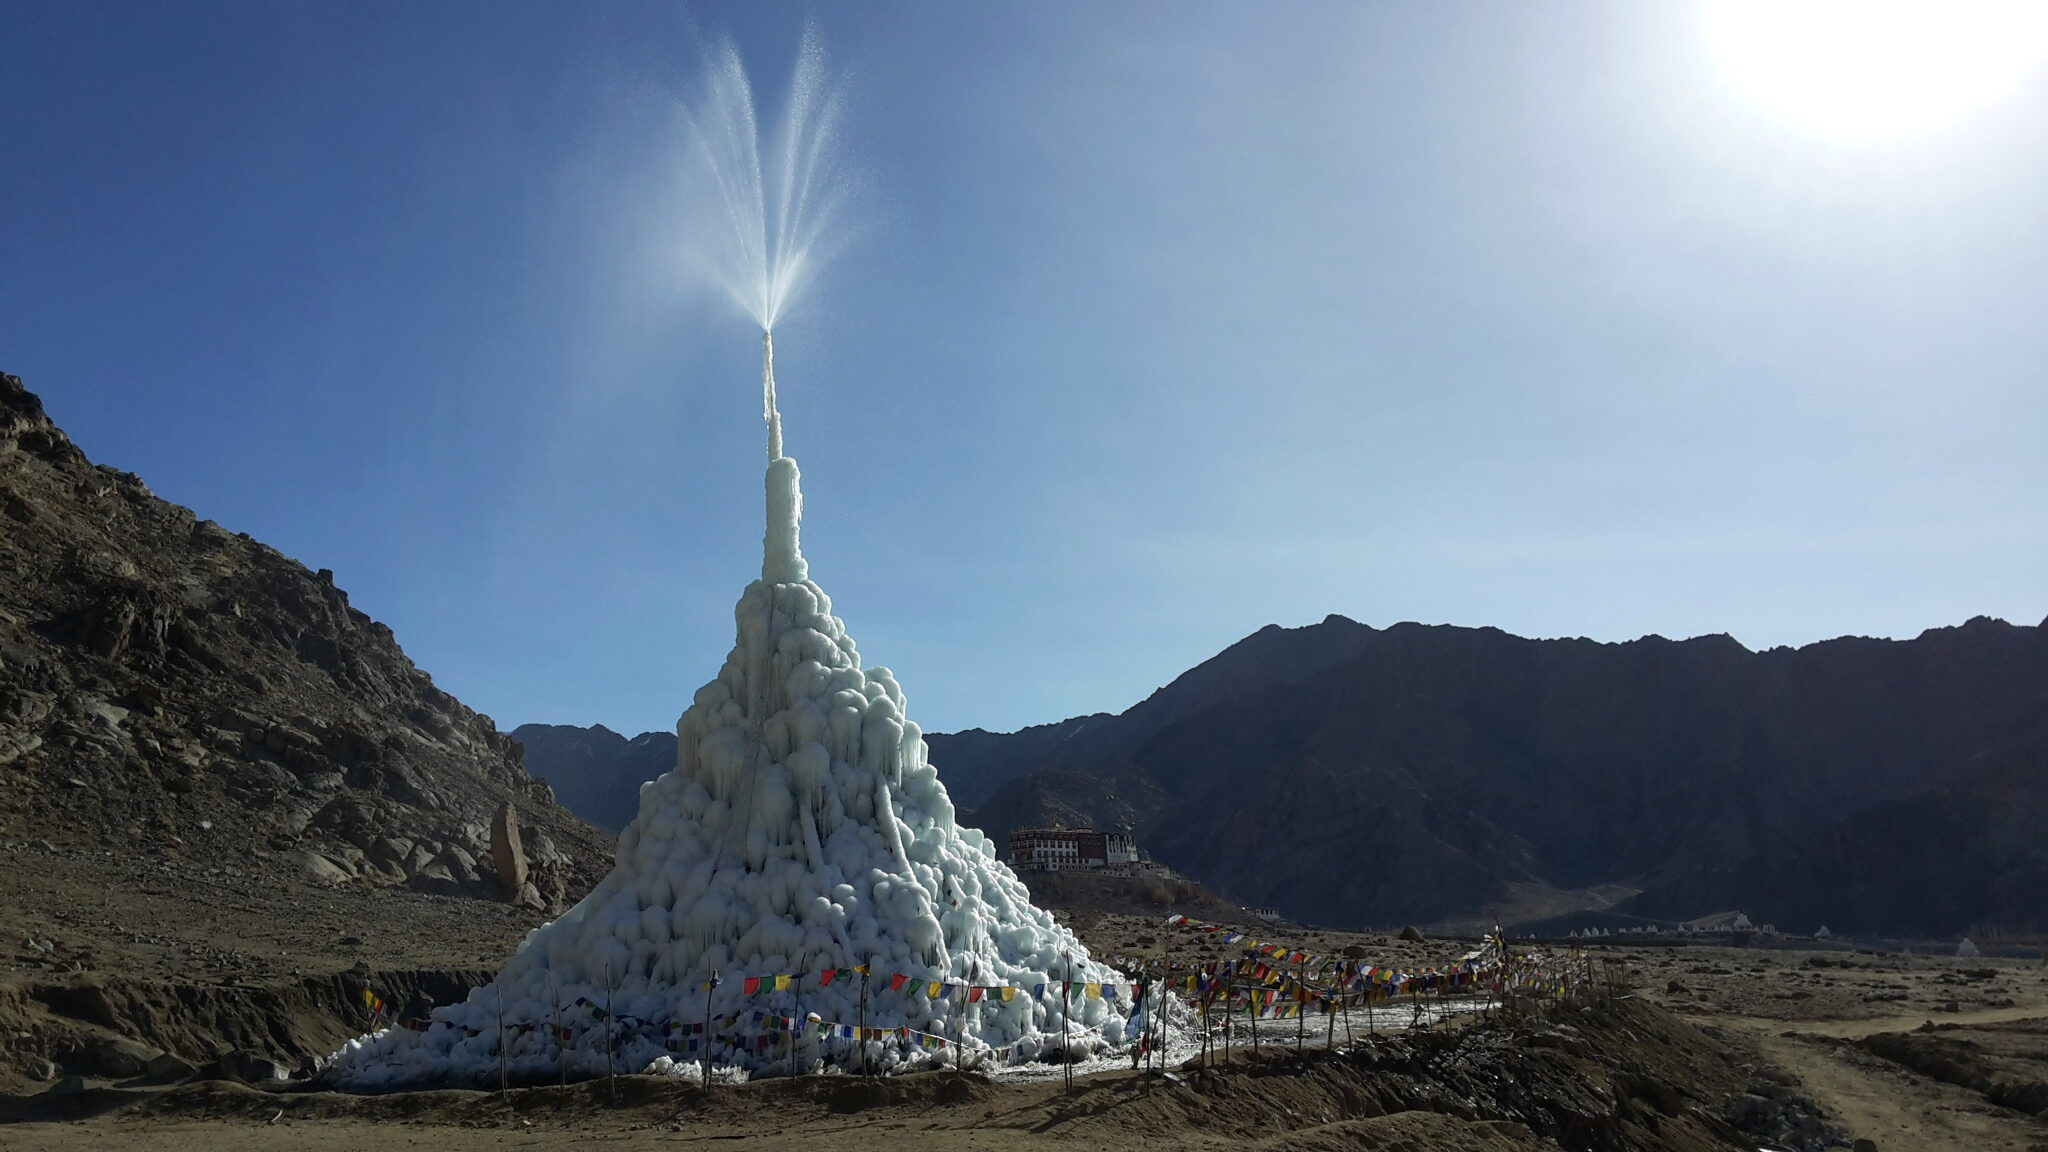
\includegraphics[width=\textwidth]{figs/IS_example.jpg}
	\caption{Ice stupa of Phyang village on March, 2015. (Photo: Sonam Wangchuk)}
	\label{fig:ISexample}
\end{figure}

Ice stupas, invented by Sonam Wangchuk in 2013, provide a much easier way to achieve water storage compared with
ice terraces \citep{wangchukIceStupaArtificial2014}. Ice stupas can be placed much closer to the plantations,
since they absorb less solar radiation per unit of volume compared with ice terraces due to their conical shape.
However, the typical volume range of ice stupas is also much smaller than that of ice terraces
\citep{nusserSociohydrologyArtificialGlaciers2019}. Over the past decade, several ice stupas have been built to
supplement irrigation water supply of mountain villages \citep{wangchukIceStupaCompetition2020,
palmerStoringFrozenWater2022, aggarwalAdaptationClimateChange2021}.


\begin{figure}[htb]
	\centering
	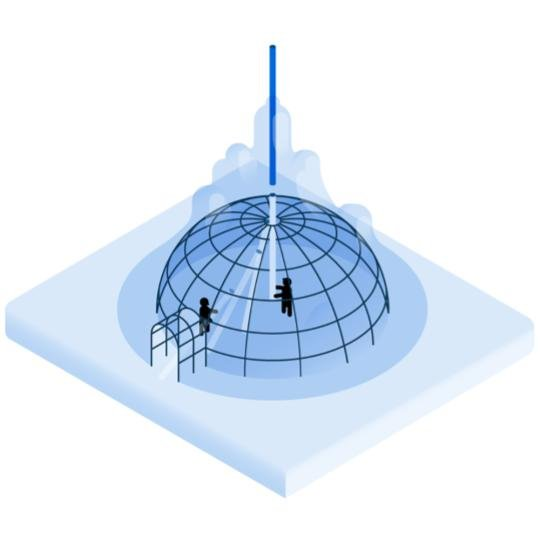
\includegraphics[width=8cm]{figs/IS_science.jpg}
	\caption{The construction process of ice stupas. Diagram by: Francesco Muzzi }
	\label{fig:ISconstruction}
\end{figure}

A typical ice stupa simply requires a fountain nozzle mounted on a supply pipeline (Fig. \ref{fig:ISexample}).
The water source is usually a glacial stream. Due to the altitude difference between the pipeline input and the
fountain output, water ejects from the fountain nozzle as droplets which freeze under subzero winter conditions.
The fountain is manually activated during winter nights. The fountain nozzle is raised by adding
metal pipes when a significant amount of ice accumulates below (Fig. \ref{fig:ISconstruction}). Typically, a dome of
branches is constructed around the metal pipes so that pipe extensions can be installed from within this dome.
Threads, tree branches, and fishing nets are used to guide and accelerate ice formation.

\subsubsection{Water storage and cost}
\label{sec:icestupa_irr}

The total cost of any water reservoir can be broken down using two activities involved, namely, transporting water into the reservoir (usually via pipelines) and constructing the physical structure that stores the accumulated water (usually concrete tanks). Ice stupas can provide cheaper water storage options since they require no physical structure to accumulate water as ice. However, their water transportation cost can be higher since they need pipelines with better insulation and larger diameters to operate during winter conditions. Typical pipeline configuration in Ladakh consists of a high-density polyethylene pipeline of 63-$mm$ diameter. Based on field estimates, the infrastructure cost of such a
system is around 6875 USD per $km$ of pipeline length.


\begin{figure}
	\centering
	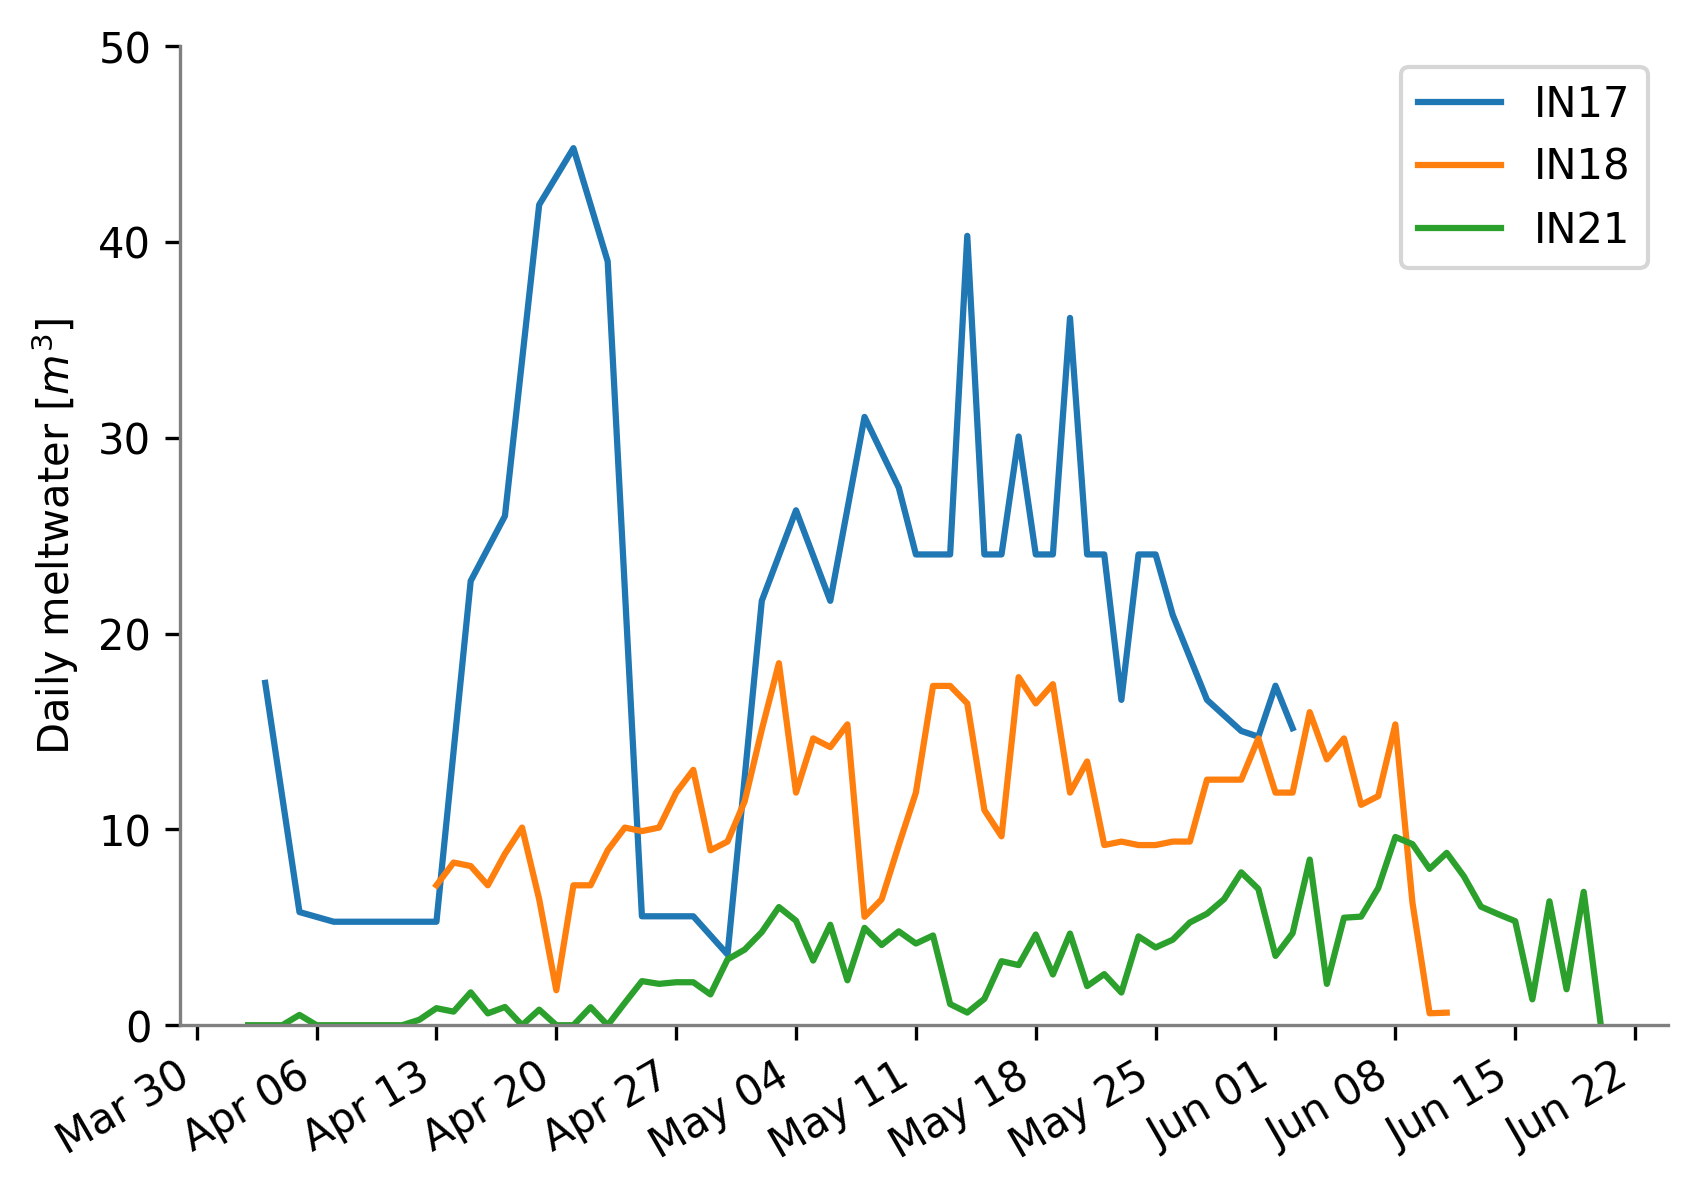
\includegraphics[width=\textwidth]{figs/melt.png}
	\caption{Daily meltwater measurements for the IN17 and IN18 AIRs along with the corresponding model estimations
		for the IN21 AIR. }
	\label{fig:ISmelt}
\end{figure}


% The cost of construction primarily depends on the material, size, and length of the pipeline required. The
% fountain nozzle's cost is negligible in comparison. 


Figure \ref{fig:ISmelt} shows the temporal variation of daily meltwater quantities obtained from three different
AIRs built in Ladakh during their melting periods (mid-April to mid-June). IN17 and IN18 AIRs were constructed
in Phyang village, and their meltwater quantities were measured manually (Fig. \ref{fig:ISirrigation}) by recording the water level of an ice stupa meltwater collection tank
\citep{vermaIceStupaMeltwater2018}. IN21 was constructed in Gangles village, and its meltwater quantities
were modelled (paper I). Differences among AIRs reflect the corresponding interannual variability in weather
conditions. The median daily AIR meltwater quantities measured were higher than 11,000 $l$.

\begin{figure}
	\centering
	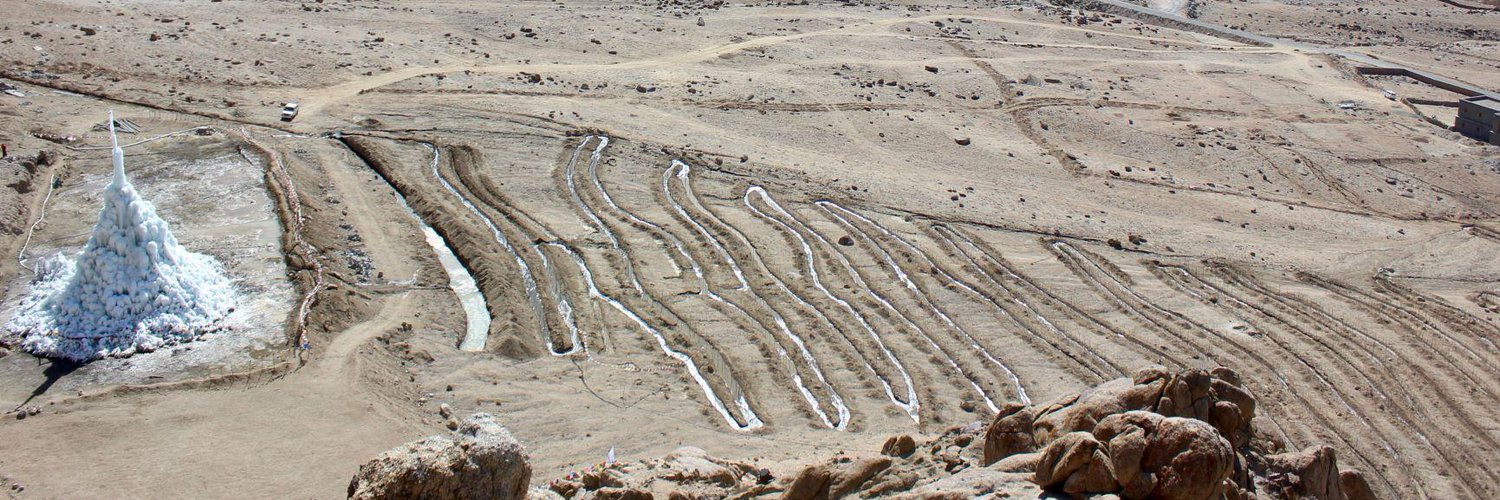
\includegraphics[width=\textwidth]{figs/IS_irrigation.jpeg}
	\caption{Irrigation channel of the ice stupa at Phyang village, Ladakh, India. (Photo: Lobzang Dadul) }
	\label{fig:ISirrigation}
\end{figure}

\section{The need for water supply management}

A common issue of AIR construction systems is water supply management: answering the questions "when to
water?", "how much?", and "for how long?". Starting water supply too early, spraying too much water, or
running water supply for too long might lead to overwatering; at the very least, this practice wastes water.
Similarly, starting the water supply too late, supplying too little water, or not running the water supply long
enough might lead to underwatering and can cause reduced ice volume. The management of water supply
differs based on the type of AIR used. The following analysis only considers the ice stupa
form of AIRs, where water supply management can also be referred to as fountain scheduling.

Paper I shows that manual ice stupa construction systems suffer from overwatering. To avoid this issue, the
energy balance models developed in the \textit{Science} chapter can be used to regulate fountain water supply
through its surface freezing rate estimations. For example, in Indian AIRs, the fountain discharge rate could
theoretically be halved since it is always twice as high as the modelled freezing rate. However, in practice, a
reduction of the discharge rate could increase the maintenance cost due to a higher risk of freezing events in
the fountain pipeline. Therefore, an optimum fountain operation strategy should first prevent the occurrence of
any freezing events. These events can be prevented by setting a minimum threshold for the recommended discharge
rate.

Adjusting fountain discharge rates in response to significant diurnal and seasonal variations of freezing rates
requires the use of automation systems. Therefore, this section describes such an automated construction
strategy that can reduce water losses and maintenance requirements compared to manual construction strategies.
First, two AIRs were built in the same location with and without automated fountain scheduling strategies; both
were measured and compared (Fig. \ref{fig:autovsman}). The associated datasets and the methods used to analyze
them are described in paper II. In a second step, differences in construction strategies between Indian and
Swiss AIRs studied in previous winters were quantified using model simulations. 

\begin{figure}[htb]
	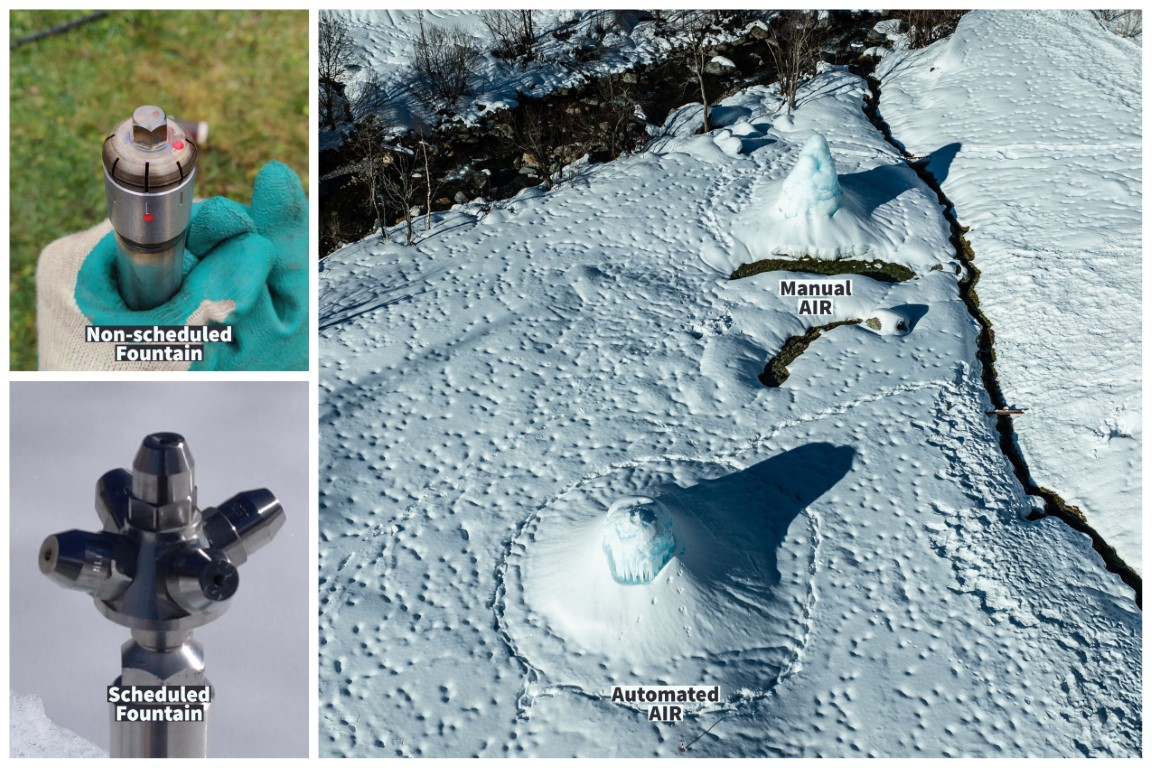
\includegraphics[width=\textwidth]{figs/AIR_fountains.jpg}
	\caption{Non-scheduled and scheduled fountains used for construction of manual and automated AIRs, respectively, at
		Guttannen. Photo: Daniel Bürki.}
	\label{fig:autovsman}
\end{figure}

\subsection{Automated fountain scheduling system}

Recommended discharge rates can only be produced if more information about the AIR surface properties and
weather conditions is available. In particular, resolving the uncertainty in the expected freezing rate requires
quantification of the following three model variables: slope, albedo, and cloudiness. However, these properties
cannot be predicted beforehand. Therefore, the upper and lower bound of each variable are associated with a
different model depending on whether these increase the freezing rate or not.  Higher slope and albedo values
decrease the shortwave radiation impact. Higher cloudiness values increase both the shortwave and the longwave
radiation impact. The model overestimating the freezing rate is referred to as \ac{IVOM}, and the model
underestimating the freezing rate is referred to as  \ac{WEOM}. Accordingly, the values
assigned to all three variables in the respective models are presented in Table \ref{tab:assumptions}.

The fountain scheduling software implements two types of fountain scheduling strategies depending on which
model type is suitable. \ac{WEOM} type is used if the location presents limited water availability, since it is expected to
produce better water-use efficiency. \ac{IVOM} type is used if the location presents limited duration of favorable
weather windows, since it is expected to produce higher ice volumes. These two types of scheduled fountains are referred to as water-sensitive fountain and weather-sensitive fountain, respectively.

\begin{table}[htb]
	\centering
	\caption{Assumptions for the parametrization introduced to simplify the ice-volume-optimized model (IVOM) and
		the water-use-efficiency-optimized model (WEOM). $\alpha_{snow/ice}$ represents albedo of snow or ice, respectively.}
	\label{tab:assumptions}
	\begin{tabular}{|lllll|}
		\toprule
		\textbf{Estimation of}          & \textbf{Symbol} & \textbf{IVOM}   & \textbf{WEOM}  &                       \\\midrule
		\multicolumn{1}{|l}{Slope}      & $s_{cone}$      & 1               & 0              & \multicolumn{1}{l|}{} \\
		\multicolumn{1}{|l}{Albedo}     & $\alpha$        & $\alpha_{snow}$ & $\alpha_{ice}$ & \multicolumn{1}{l|}{} \\
		\multicolumn{1}{|l}{Cloudiness} & $cld$           & $0$             & $1$            & \multicolumn{1}{l|}{} \\\bottomrule
	\end{tabular}
\end{table}

The assumptions described in Table \ref{tab:assumptions} are applied on the one-dimensional description of
energy fluxes through Eqn. \ref{eqn:EB}. The derivation of the individual energy and mass balance terms for the
\ac{IVOM} and \ac{WEOM} versions are discussed in the Appendix \ref{sec:auto_software}.

\begin{figure}
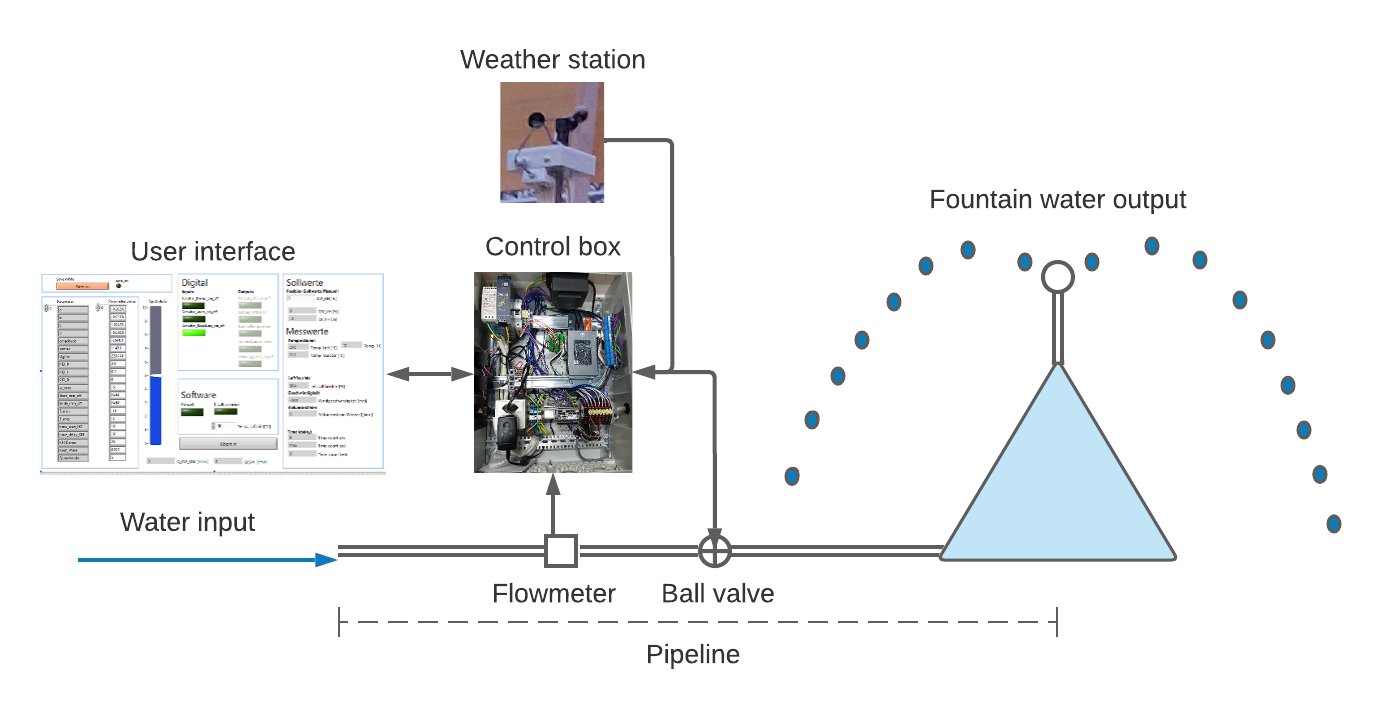
\includegraphics[width=\linewidth]{figs/Automation_schematic.png}
\caption{Schematic illustrating the measurement and control of the fountain pipeline system through the
  automation system. Two-way arrows indicate information exchange between different components whereas one-way
  arrows indicate information transmission.}

\label{fig:auto_schematic} 
\end{figure}

Equation \ref{eqn:EB} is implemented in the automation software. The user interface of the software enables
input of the spray radius, altitude, latitude, and longitude of the construction location. The automation
hardware consists of an \ac{AWS}, control box, flowmeter, ball valve, drain valves, air valves, fountain and a
pipeline (Fig. \ref{fig:auto_schematic}). The control box feeds the AWS data to the automation software to
obtain the recommended discharge rate. Then, to match this recommendation, it adjusts the ball valve position
based on the information from the flowmeter. In case a termination criterion gets met, the drain and air valves
are opened to allow removal of water and entry of air in the pipeline, respectively.

The recommended discharge rate is equal to the mass change rate. However, certain termination criteria listed
below override the discharge rate recommendation and drain the pipeline to prevent water loss or fountain
freezing events:

\begin{itemize}

	\item High water loss is assumed when wind speed is greater than the user-defined critical wind speed.

	\item High risk of fountain freezing event is assumed when mass change rate is lower than the user-defined minimum fountain discharge rate.

	\item Freezing events in the fountain pipeline are assumed when measured discharge rate is zero for at least
    20 seconds.

	\item Pipeline leakage is assumed when measured discharge rate is greater than the user-defined maximum fountain discharge rate.

\end{itemize}

\subsection{Comparison of manual and automated construction strategies}

\begin{figure*}[htb] 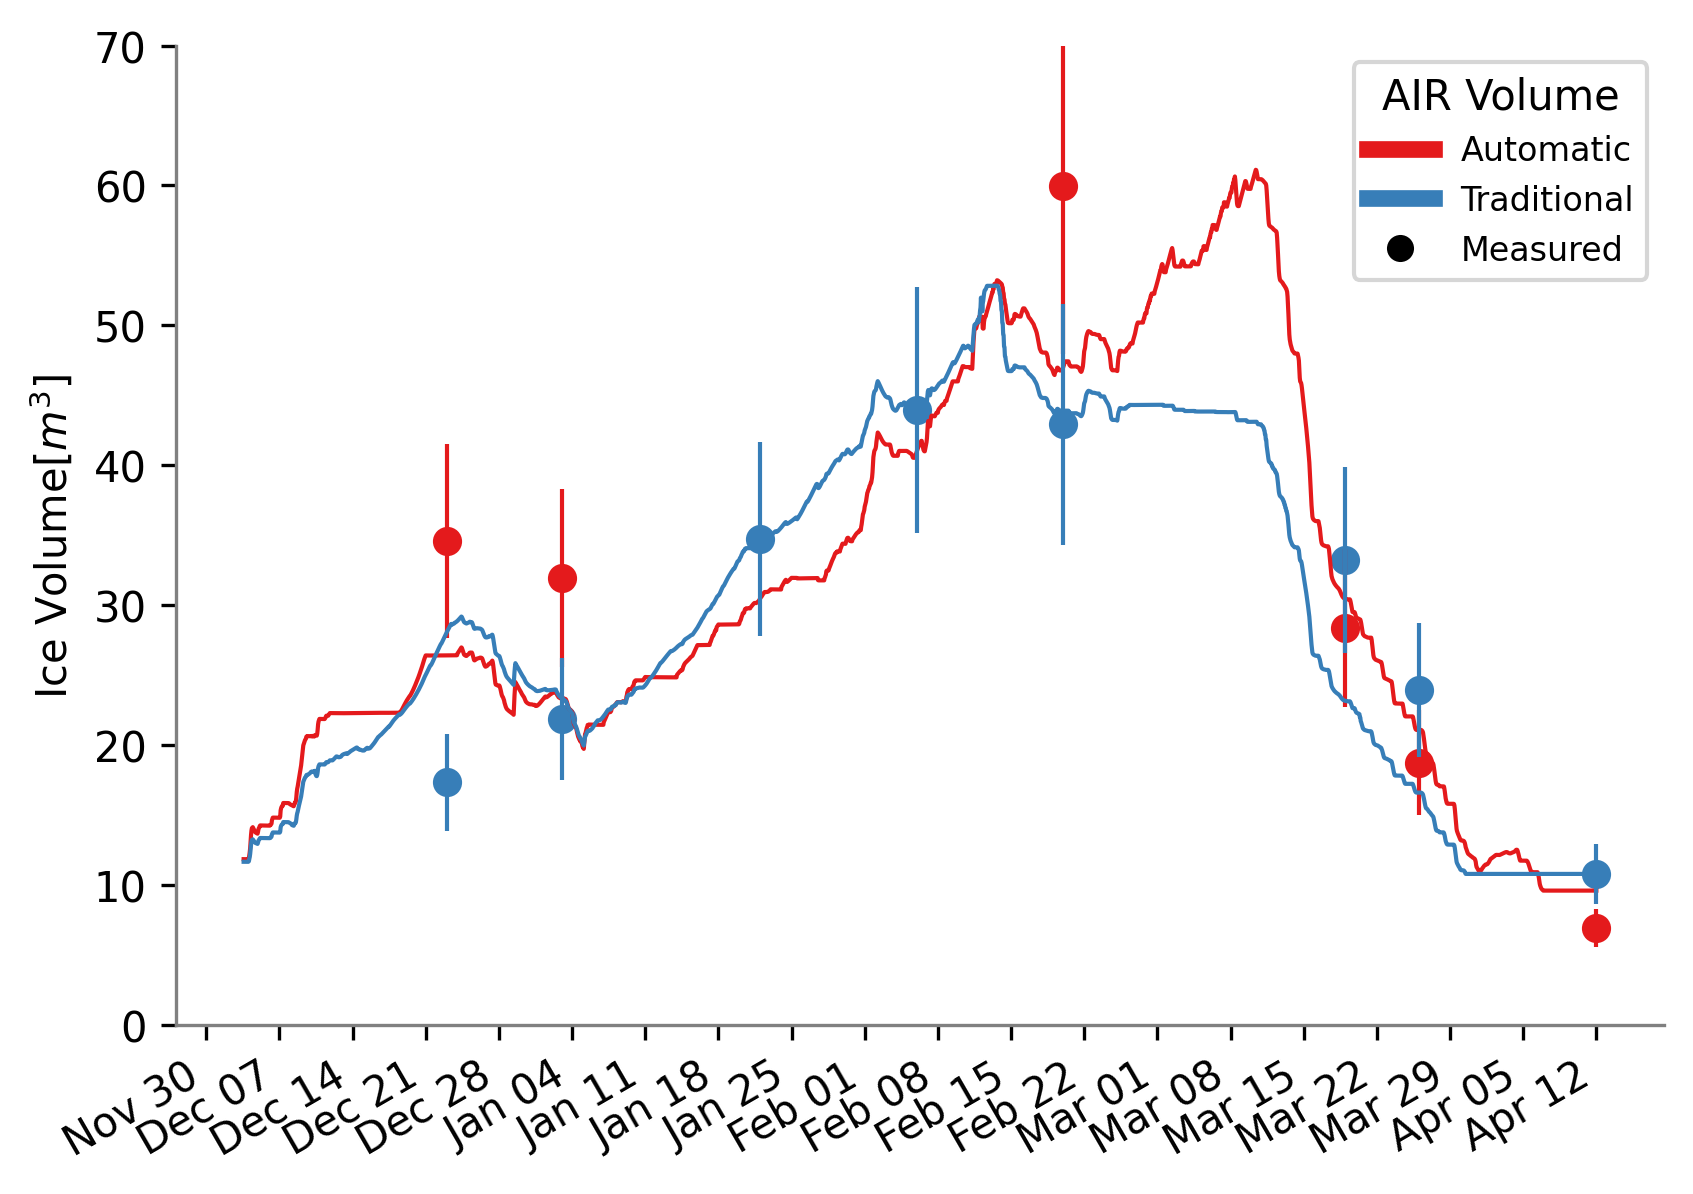
\includegraphics[width=\textwidth] {figs/CH_validation.png} \caption{Volume validation of the
		scheduled and non-scheduled fountain construction strategies.} \label{fig:validation} \end{figure*}

Fountain scheduling reduced the fountain discharge input and fountain wastewater output by an order of
magnitude. However, this did not result in an appreciable difference in the volume evolution of the automated
or the manual AIR, as shown in Fig. \ref{fig:validation}. This is due to two counteracting surface processes
during fountain spray: process A consists in the dampening of albedo to ice albedo, and process B consists in the
absorption of heat energy from the fountain water droplets. The temporal variation of the magnitude of these
processes is shown in Fig. \ref{fig:dis_processes}.

\begin{figure*}[htb]
	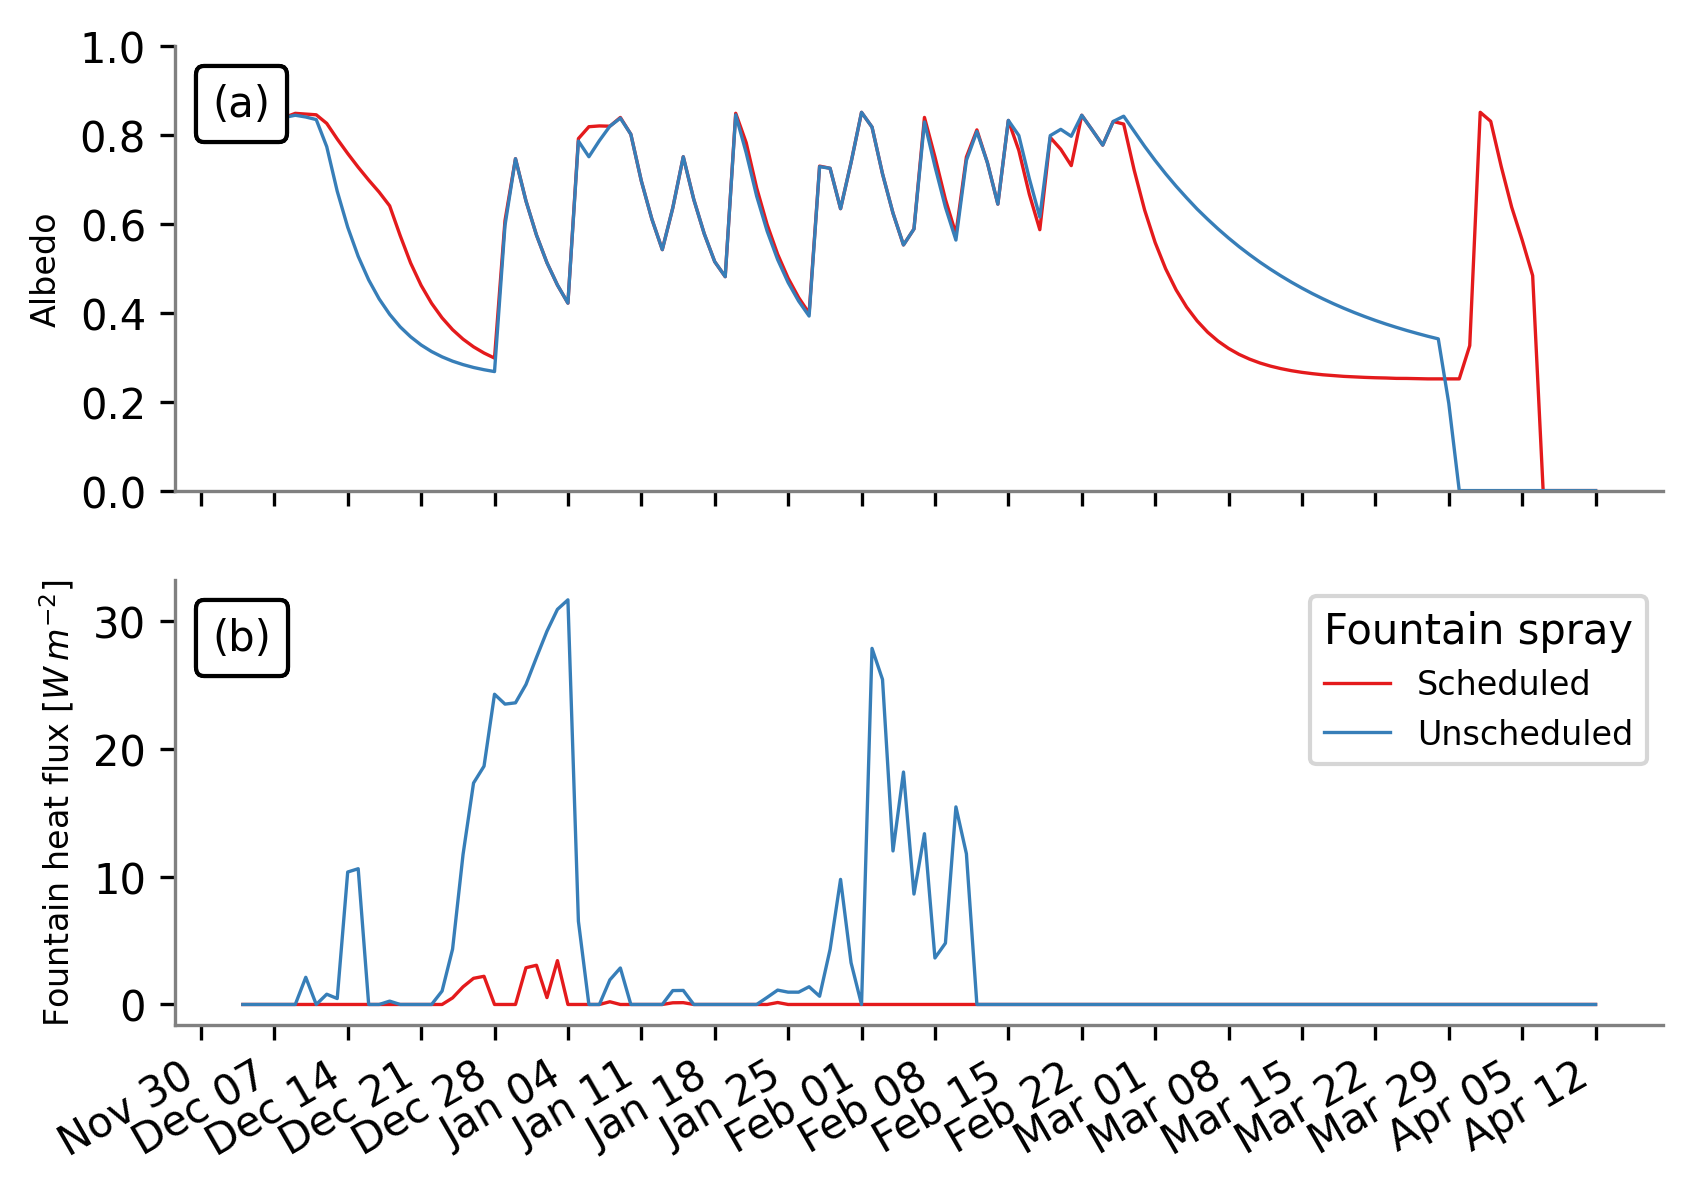
\includegraphics[width=\textwidth]{figs/dis_processes.png}
	\caption{(a) Surface albedo  and (b) fountain discharge heat flux showed significant variations between the two
		\ac{AIRs} due to the differences in their discharge rates.}
	\label{fig:dis_processes}
\end{figure*}

The difference in water-use efficiency and maximum ice volume between non-scheduled and scheduled fountains in the
Indian and Swiss locations across two winters is shown in Fig. \ref{fig:wue}a. Four experimental values
(highlighted in circles) and five simulated values (highlighted in squares) are shown together. The
experimental values were taken from the IN21 and CH21 AIRs studied in paper I and from the CH22 AIR investigated in
paper II.

\begin{figure}[htb]
	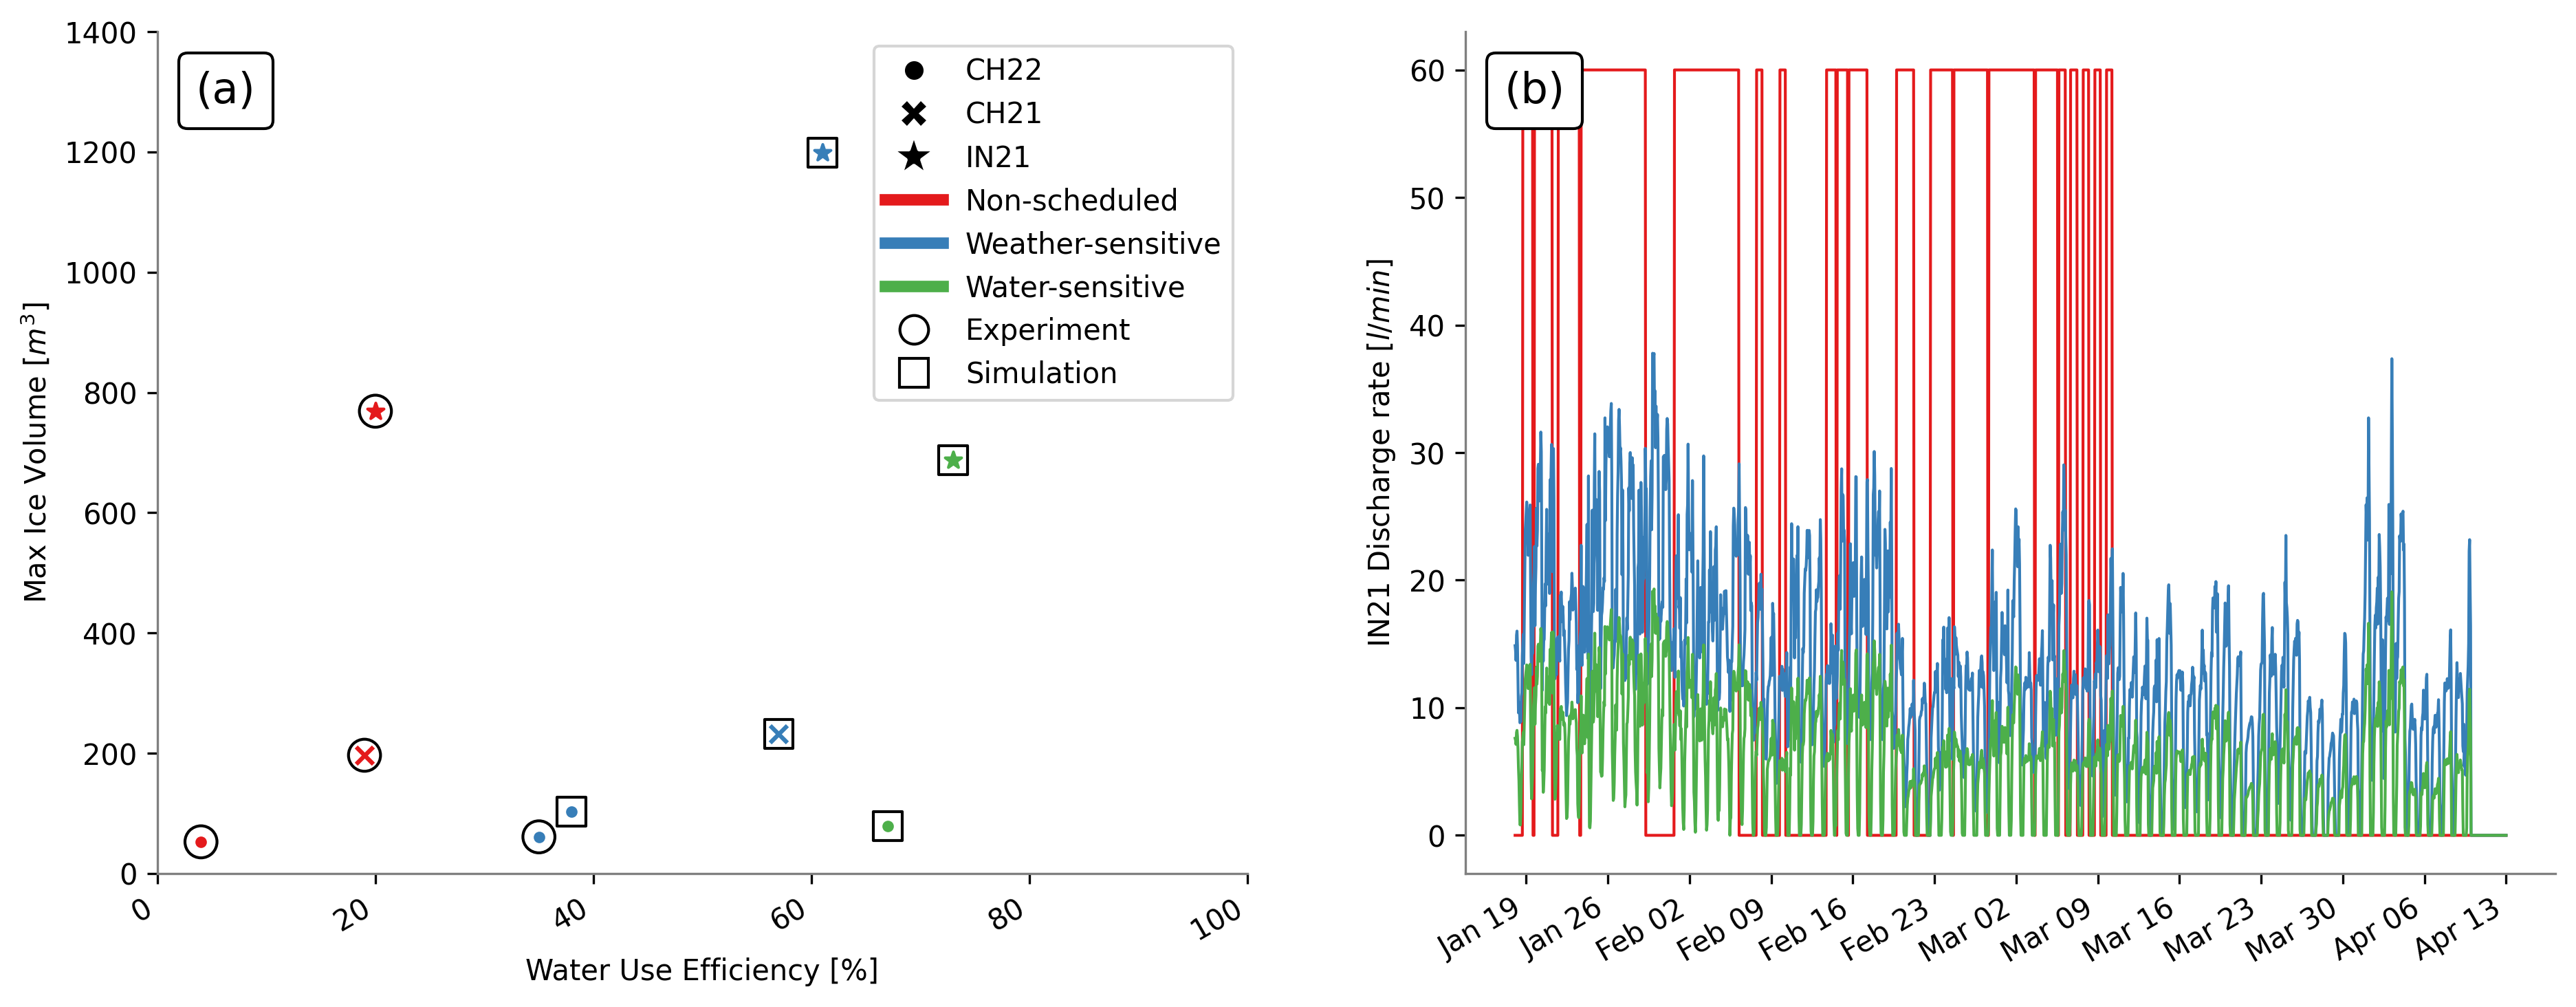
\includegraphics[width=\textwidth]{figs/wue.png}

	\caption{(a) The maximum volume and water-use efficiency estimated for AIRs constructed in different locations
		(represented by symbols) with different fountain scheduling strategies (represented by colors). Experimental
		values are highlighted in circles, and simulated values are highlighted in squares. (b) Comparison of
		the non-scheduled and scheduled fountain discharge rates at the IN21 location.}

	\label{fig:wue}
\end{figure}

Water-use efficiency of all the non-scheduled fountains is below 20\%. In general, water-use efficiency
exhibits a threefold increase when the weather- or water-sensitive fountains are used in both
locations.

For the Indian location, the three different kinds of fountains yielded significantly different results owing to discharge
duration and maximum discharge rate
(Fig. \ref{fig:wue}b). The non-scheduled fountain showed a maximum discharge rate more than twice that of
the scheduled fountains, resulting in higher water loss; freezing events in its pipeline caused frequent
interruptions in the non-scheduled discharge rate (Fig. \ref{fig:wue}b). In contrast, mean freezing
rates of the other two fountains during these events were above their median values. This is because very cold
temperatures freeze the water inside rather than outside the fountain system, instigating such freezing events in
the fountain pipeline. Therefore, the discharge duration of the non-scheduled fountain was much lower, resulting in
lower ice volume. The water-sensitive fountain underestimated the freezing rate during the construction period
and therefore produced much lower ice volume compared with the weather-sensitive fountain.

For the Swiss locations, scheduled fountains yielded better water-use efficiency but did not significantly alter
the maximum volume obtained.

